\begin{figure}
  \centering
  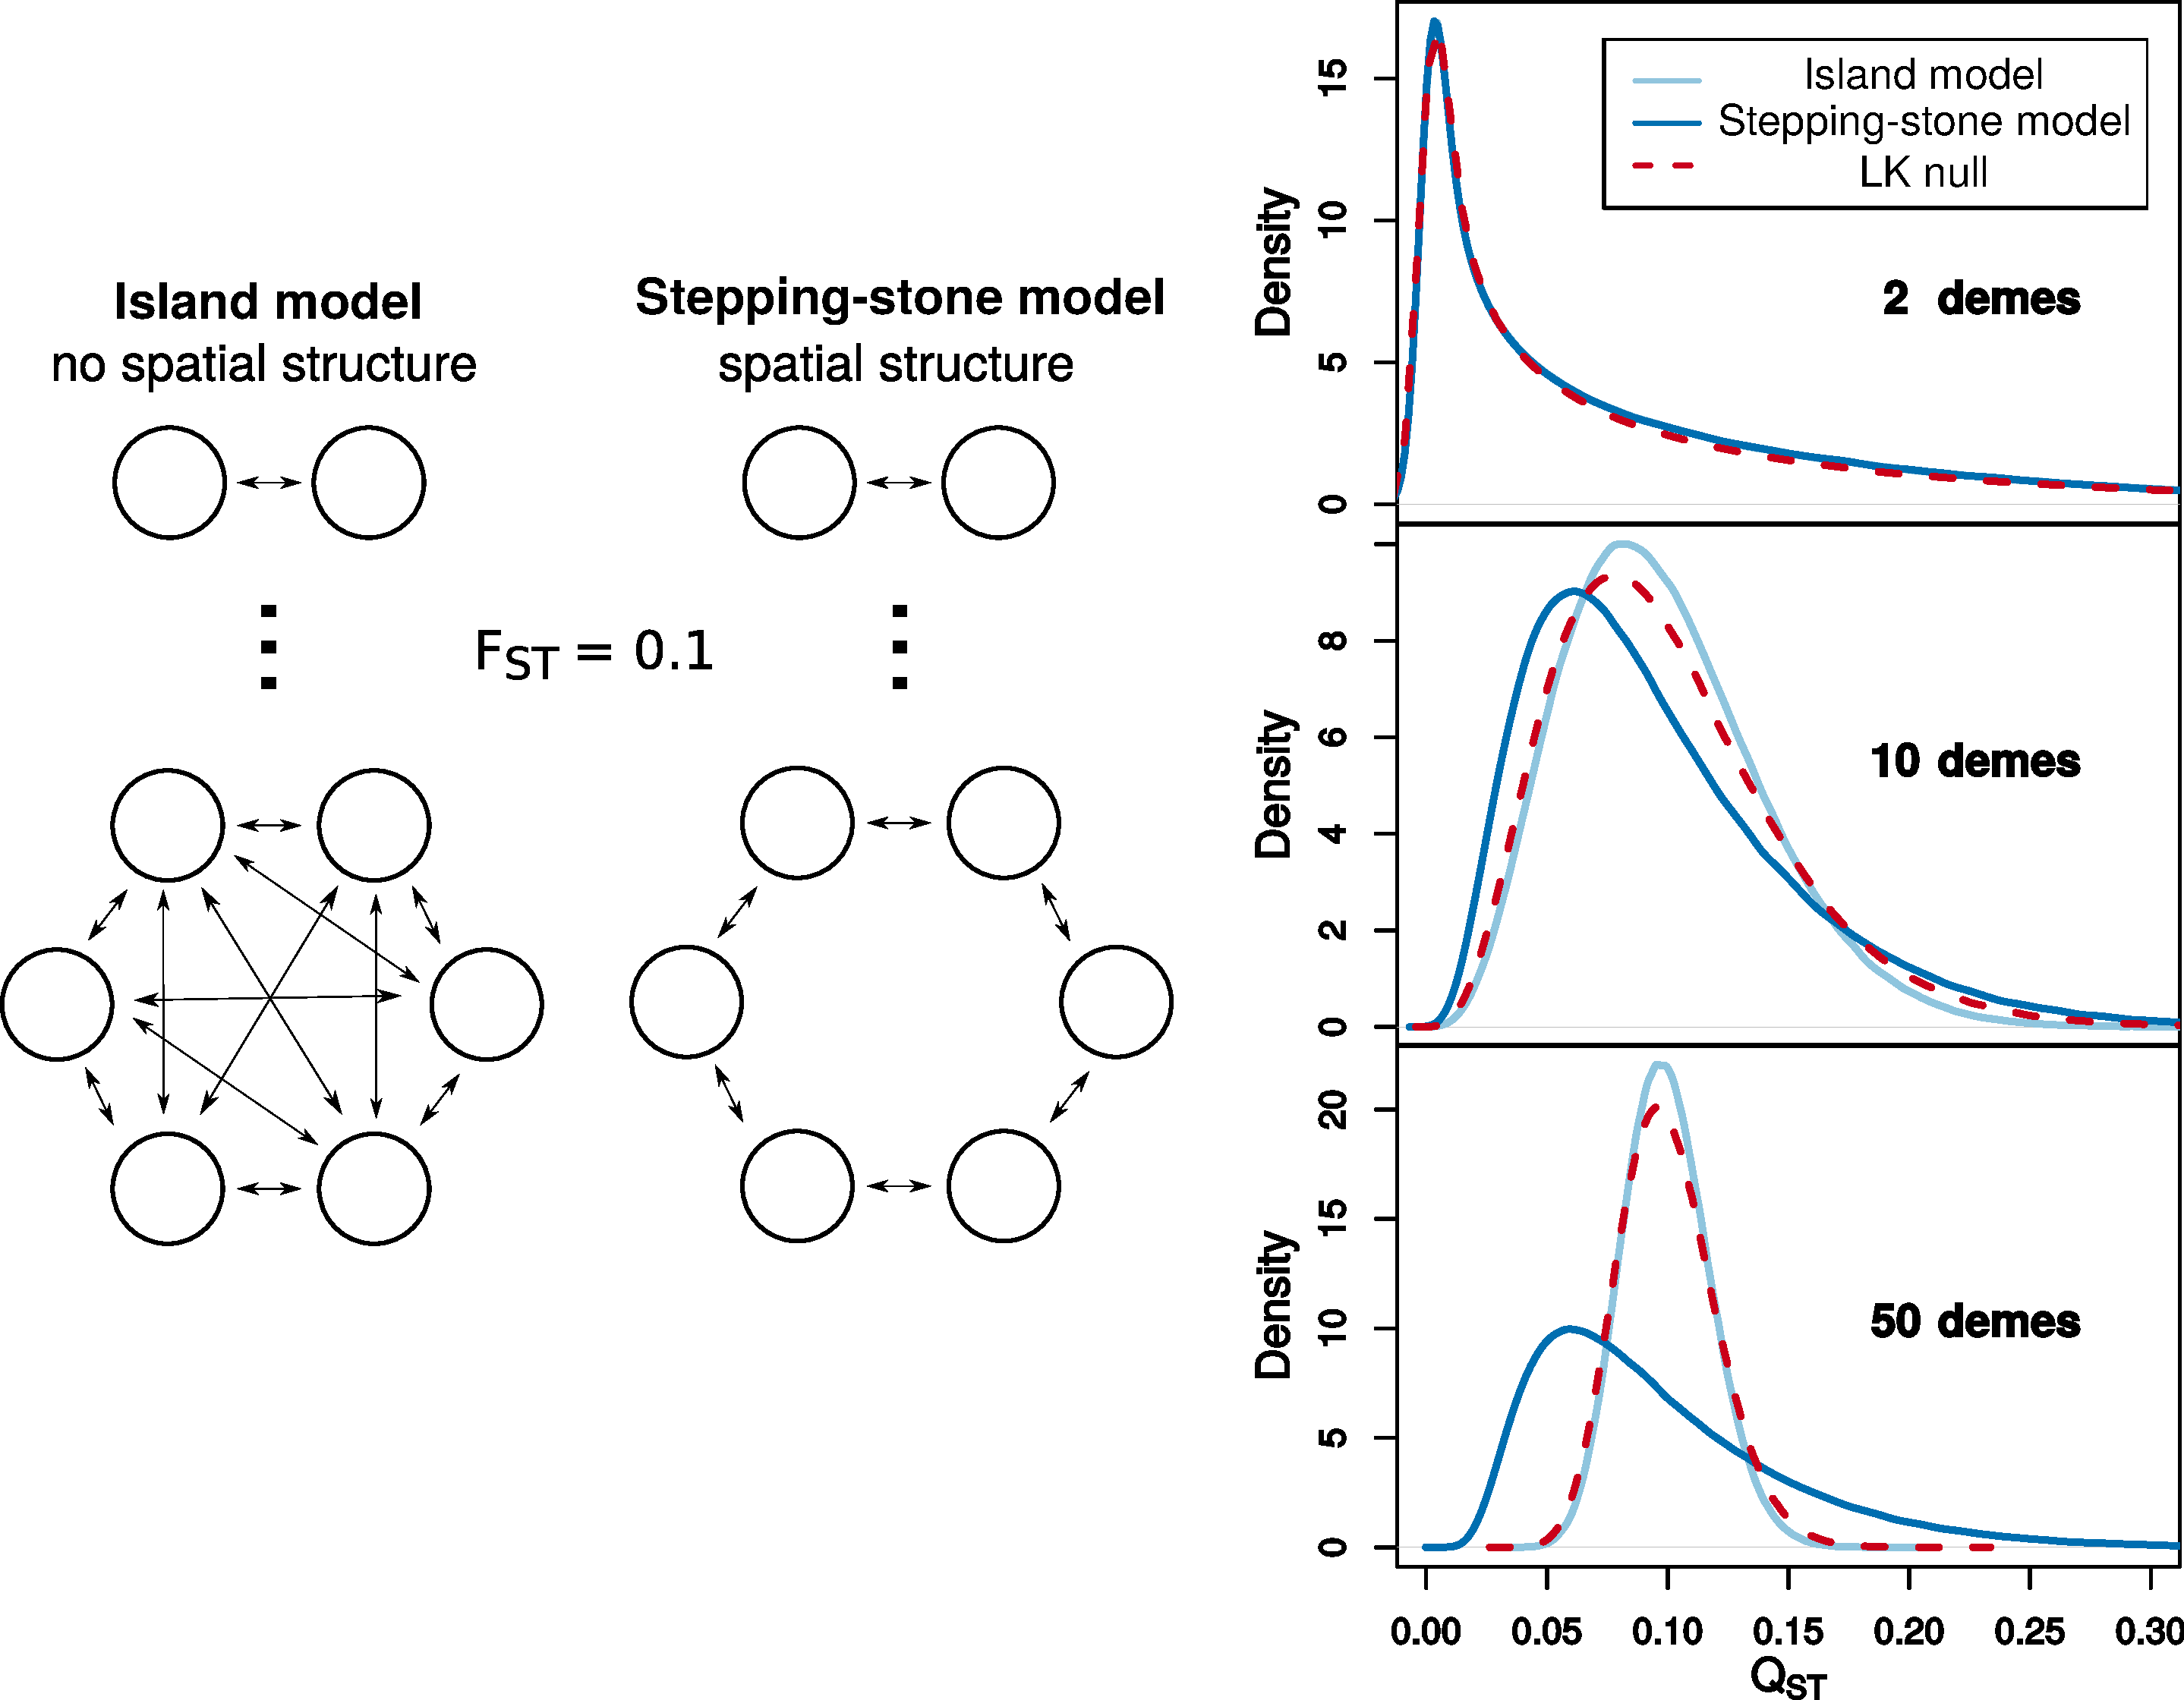
\includegraphics[width=0.95\textwidth]{./figures/pop_struct_combine_alt.pdf}
  \caption{ \textbf{A comparison of neutral sampling distributions for $Q_{ST}$
      at the population level.} The Lewontin-Krakauer (LK) distribution for
    $Q_{ST}$ is compared to the null distribution in the infinitesimal limit for
    cases with (the stepping-stone model) and without (the island model) spatial
    structure. The case with no spatial structure assumes the migration rate is
    equal between all subpopulations. The case with spatial structure arranges
    subpopulations in a ring with migration only between neighboring
    subpopulations. Migration rates and subpopulation sizes are uniform and are
    set such that $F_{ST}=0.1$ as the number of subpopulations increases
    \citep{Slatkin1991}. $Q_{ST}$ values for these models are simulated by
    drawing vectors from a multivariate normal distribution parameterized using
    the expected pairwise coalescence times given by \citep{Slatkin1991}. Under
    the LK distribution $Q_{ST}$ is distributed as $F_{ST}/(n_d - 1)$ times a
    chi-square distribution with $n_d - 1$ degrees of freedom ($Q_{ST}\sim
    F_{ST}\chi^2_{n_d - 1}/(n_d-1)$), where $n_d$ is the number of
    subpopulations. The neutral distributions for
    $Q_{ST}$ become increasingly different as the number of subpopulations over
    which the genetic divergence is spread increases.}
  \label{fig:qst_deme}
\end{figure}
\begin{figure}
  \centering
  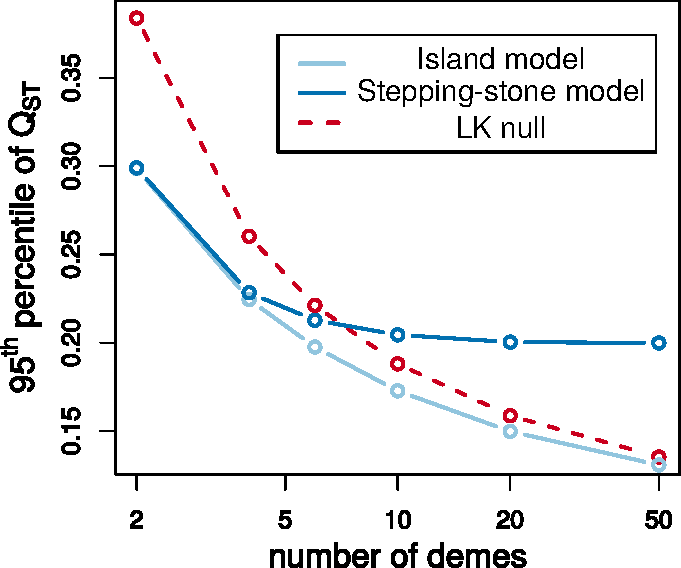
\includegraphics[width=0.5\textwidth]{./figures/qst_deme_percentile_nospace_alt.pdf}
  \caption{\textbf{Differences in the $95^{\mathrm{th}}$ percentile of different
      neutral sampling distributions for $Q_{ST}$ at the population level.} The
    Lewontin-Krakauer (LK) distribution is compared to neutral null
    distributions for structured populations with and without a spatial
    component using the normal model arising in the infinitesimal limit.}
  \label{fig:qst_perc}
\end{figure}


To demonstrate the utility of the normal distribution arising in the
infinitesimal limit (equation \ref{eq:normcov}), we use simulating from the null
distribution of $Q_{ST}$, a measure of divergence in trait values between groups
in structured populations. $Q_{ST}$ is defined as the variance between group
means divided by the total variance in the population \citep{Spitze1993}. In a
haploid model, $Q_{ST} = \frac{V_{between}}{V_{between} + V_{within}}$, where
\begin{equation*}
  V_{between} = \frac{1}{K} \sum_i \left( \bar{Y}_i - \bar{Y} \right)^2
\end{equation*}
and
\begin{equation*}
  V_{within} = \frac{1}{\sum_k N_k} \sum_i \sum_j \left( Y_{i,j} - \bar{Y}_i \right)^2.
\end{equation*}
Here, $Y_{i,j}$ is the trait value of individual $j$ in population $i$, $K$ is
the number of subpopulations, and $N_k$ is the size of subpopulation $k$.

Since all $Y_{i,j}$ are normally distributed, $\bar{Y}_{i} - \bar{Y}$ and
$Y_{i,j} - \bar{Y}_i$ are as well. When population sizes are large, individual
deviations from population means are nearly uncorrelated, as are $V_{between}$
and $V_{within}$. $V_{within}$ is nearly constant across evolutionary
realizations and is approximately $\sum_k N_k E[\mathcal{T}_{k,k}] / \sum_k N_k$
because the within population variances are approximately uncorrelated and
constant. While we do not have an explicit form for the density function of the
between-group variance, we can simulate from its distribution by drawing
$\bar{Y}_{i} - \bar{Y}$ values from a multivariate normal distribution with mean
zero and covariance
\begin{equation}
  \Cov[\bar{Y}_{a} - \bar{Y}, \bar{Y}_{b} - \bar{Y}] =
  \mu_2 \T (\E[\mathcal{T}_{a,\cdot}] + \E[\mathcal{T}_{b,\cdot}] -
  \E[\mathcal{T}_{\cdot,\cdot}] - \E[\mathcal{T}_{a,b}])
\end{equation}
between populations $a$ and $b$. To simulate from the null distribution of
$Q_{ST}$, $\mu_2$ and $\T$ are unnecessary because the scale of the trait
cancels in the $Q_{ST}$ ratio. All that is needed to simulate $Q_{ST}$ are the
relative expected coalescent times within and between populations which can be
estimated using pairwise nucleotide differences. No further information about
population structure, history, or mutation rate is needed.

This simulation procedure could be useful in testing whether an observed
$Q_{ST}$ is unlikely under neutrality. Current goodness-of-fit tests either
compare $Q_{ST}$ to an empirical distribution of $F_{ST}$ values or to a
$\chi^2$ distribution \citep{Leinonen2013}. In the second case, a distribution
developed by \citet{Lewontin1973} for single-locus neutrality tests is used as
the null distribution for $Q_{ST}$. The $\chi^2$ testing procedure was suggested
by \citet{Whitlock2009} and is implemented in the program \textit{QstFstComp}
\citep{Gilbert2015}. The Lewontin-Krakauer (LK) distribution assumes
independence between subpopulations and provides a good approximation in
populations without spatial structure, such as in a symmetric island model
(Figure \ref{fig:qst_deme}). When subpopulations are strongly correlated, such
as in a one-dimensional stepping-stone model, the LK distribution is a poor
approximation. Even when the distributions appear qualitatively similar, there
are substantial differences in tail probabilities (Figure \ref{fig:qst_perc}).

Nearly identical issues to these were raised with the LK test
\citep{Nei1975,Robertson1975}. However, while the neutral distribution for
$F_{ST}$ depends on the precise details of population structure and history, the
$Q_{ST}$ distribution only depends on coalescence times within and between
subpopulations. The point here is not that the LK distribution is particularly
bad, but rather that an improved neutral distribution is easily obtained using
the infinitesimal limit. This distribution is similar to the extension of the LK
test developed by \citet{Bonhomme2010} to account for the correlation structure
between subpopulations. The \citet{Bonhomme2010} method treats allele
frequencies as multivariate normal with covariance matrix parameterized by
coancestry coefficients. \citet{Ovaskainen2011} and \citet{Berg2014} use normal
models for phenotypes also with covariance matrices based on coancestry
coefficients. When phenotypic and genetic divergence is mostly driven by changes
in allele frequency, the coalescent and coancestry based models should be very
similar. However, the coalescent model is ultimately preferable since it is the
correct neutral model at any scale of population divergence in the infinitesimal
limit. A coancestry model is the only option if only allele frequency data are
available, but it is still better to use the full matrix of coancestry than to
use a single value of $F_{ST}$.

Treating $Q_{ST}$ as a random variable also lets us reexamine the classic result
in evolutionary quantitative genetics that $Q_{ST}=F_{ST}$ \citep{Whitlock1999}.
$F_{ST}$, in this context, refers to a population parameter. In particular,
$F_{ST} = \frac{\bar{t} - \bar{t}_0}{\bar{t}}$, where $\bar{t}$ is the expected
coalescent time for two loci sampled at random from the entire population and
$\bar{t}_0$ is the expected coalescent time for two loci sampled within a
subpopulation \citep{Slatkin1991}. This value is constant over realizations of
the evolutionary process. $Q_{ST}$ can refer to either the state of the
population or to an estimate of this state. $Q_{ST}$, as a state of the
population, varies across evolutionary realizations. Thus, there is no sense in
which $Q_{ST}$ can be defined as a constant parameter in the way that $F_{ST}$
can. The expectation of $V_{between}$ is $\bar{t} - \bar{t}_0$, and the
expectation of $V_{within}$ is $\bar{t}_0$.
$\frac{\E[V_{between}]}{\E[V_{between}] + \E[V_{within}]}$ is equal to $F_{ST}$.
Due to Jensen's inequality, the expectation of this ratio ($\E[Q_{ST}]$) is
never greater than $F_{ST}$. This was previously shown by \citet{Edge2015} for a
slightly different trait model.

%%% Local Variables:
%%% TeX-master: "quant_gen_manu.tex"
%%% End:
